\subsection{Power Measurement and Acquisition Setup}
\CC{Jayant writes this. You can start with the text below which is what Aakarsh wrote and modify it according to the setup you used. Also include a good picture.}
\begin{figure}[t]
  \centering
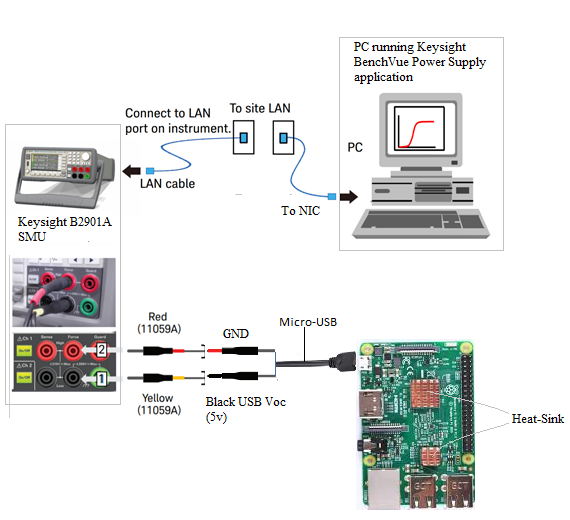
\includegraphics[width=0.9\columnwidth, height=8cm]{expsetup}
  \caption{Experimental Framework}\label{expsetup}
\end{figure}
Fig.~\ref{expsetup} describes our experimental framework to measure the power and performance characteristics of various constituent obfuscation techniques along with the data acquisition system. We utilize the Raspberry Pi which is a popular platform for low-power and low-cost computational tasks with widespread applications as our resource constraint device. With it's support for input-output peripherals, network connectivity and programmability, it is exemplary for IoT applications~\cite{maksimovic2014raspberry}.

In our setup, we utilize the Raspberry Pi 3 Model B+ (RPi) running Broadcom BCM2837B0, quad-core A53 (ARMv8) 64-bit SoC @1.4GHz processor, 1GB LPDDR2 SDRAM with 5V/2.5A DC input power via microUSB connector and operating temperature between 0 to $60^{\circ}C$.


\CC{Jayant and Aakarsh: rewrite this to fit our current system.}
We have built a custom setup to measure the power consumption from the RPi3 . The RPi3 is powered via a microUSB from a stable 5V/2.5A power supply . (Fig.~\ref{expsetup}), from which the power consumed by the RPi $P$ = $V\times I$.
For providing the required power supply to Pi and capturing the power drawn due to obfuscated code execution, we make use of highly accurate source meter unit i.e. Keysight SMU. We use 2-wire connection with SMU kelvin probes to a open ended micro usb 2-wire cable which in turns powers the Raspberry Pi with constant and accurate power supply which we have specified to be 5V/2.5A max as per Pi 3 specification.
There is a connection between the SMU and a PC via LAN cable to control the SMU via Keysight command and control application to extract the required current(I) and voltage(V) values from the SMU to the desktop application called as Keysight BenchVue Power Supply. 

The Raspberry Pi 3 has an on-chip temperature sensor that measures the temperature (T) of the CPU. This provides additional information of the heat state of the Raspberry Pi. We used 2 heat-sinks, external cooling fan in an air conditioned environment to maintain the temperature of the Pi. Ideally the temperature should be between $0^{\circ}C$ to $60^{\circ}C$ for the optimal working state of the Pi whereby the heat does not affect calculations of  execution time values which are themselves averaged over 5 executions of the obfuscated targets.

The obfuscated target outputs generated, as in ~\ref{subsec:pdoc} are executed on the Pi and power samples are acquired on the laptop.
`'